\documentclass[12pt]{article}

\usepackage[margin=1.9cm, letterpaper]{geometry}
\usepackage[utf8]{inputenc}
\usepackage{indentfirst}
\usepackage{tikz}
\usepackage{float}
\usepackage{subcaption}
\usepackage{amsmath}
\usepackage{amssymb}
\usepackage{booktabs}
\usepackage{siunitx}
\usepackage{pdfpages}
\usepackage{minted}
\usepackage{fontspec}
\usepackage{hyperref}
\usepackage[style=ieee]{biblatex}

\setmainfont{Noto Serif}
\setsansfont{Segoe UI}
\setmonofont{Consolas}

\usetikzlibrary{arrows,automata,positioning}

\begin{document}
\begin{titlepage}
  \begin{center}
    \vspace*{1cm}

    \textbf{LAB 2}

    \vspace{0.5cm}

    Finite State Machines in VHDL

    \vspace{1.5cm}

    \textbf{Michael Kwok (1548454)}

    \vfill

    ECE 410 -- Advanced Digital Logic Design\\
    Department of Electrical and Computer Engineering\\
    University of Alberta\\
    October 20, 2021

  \end{center}
\end{titlepage}

\tableofcontents

\pagebreak

\section{Abstract}

This lab had the implementation of a sequence detector and vending machine using a Mealy machine.
For both designs, multiple VHDL processes were used as a method to improve modularity in the code, and to allow for the
synthesis tool to recognize the State Machine. An external seven-segment display was used in the 2nd part of the lab,
which required knowledge about the pinouts of the Zybo board and the connections of the seven-segment PMOD module.

\section{Design}

\subsection{Sequence Detector}
\begin{figure}[h]
  \centering
  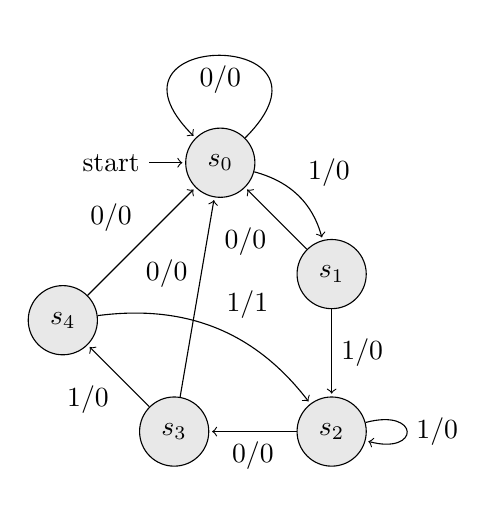
\begin{tikzpicture}[shorten >=1pt,node distance=2cm,auto]
    \tikzstyle{every state}=[fill={rgb:black,1;white,10}]

    \node[state,initial] (s_0) {$s_0$};
    \node[state] (s_1) [below right of=s_0] {$s_1$};
    \node[state] (s_2) [below of=s_1] {$s_2$};
    \node[state] (s_3) [left of=s_2] {$s_3$};
    \node[state] (s_4) [above left of=s_3] {$s_4$};

    \path[->]
    (s_0) edge [loop] node {$0/0$} ()
    (s_0) edge [bend left] node {$1/0$} (s_1)
    (s_1) edge node {$1/0$} (s_2)
    (s_1) edge node {$0/0$} (s_0)
    (s_2) edge [loop right] node {$1/0$} ()
    (s_2) edge node {$0/0$} (s_3)
    (s_3) edge node {$0/0$} (s_0)
    (s_3) edge node {$1/0$} (s_4)
    (s_4) edge [bend left] node {$1/1$} (s_2)
    (s_4) edge node {$0/0$} (s_0);
  \end{tikzpicture}
  \caption{State diagram for sequence detector}
  \label{fig:state-diagram}
\end{figure}

The first part of the lab required the design of a finite state machine to detect the sequence \verb|11011| with overlap detection. A Mealy machine was chosen for the design of this part, as it is likely to be easier than a Moore machine.

The design of the sequence detector started with the construction of a state diagram (Figure \ref{fig:state-diagram}), indicating all the present states, expected input and output combinations, and next states.
This was then implemented as a two-process behavioural model in VHDL, with one clocked process for state changes and synchronous resets and the second process handling input, state changes and output behaviour. This was done to improve the readability of the code and to more closely model what the digital logic circuit implementing the behaviour would be structured physically.

\subsection{Vending Machine}

For the second part of the lab, a ``vending machine'' was to be designed. The system accepted inputs indicating the requested item and the amount of money inserted. The system also had outputs indicating the amount of money currently inside the machine, the item dispensed, and the change returned. This part was also implemented with a Mealy machine as it reduces the number of states required.

The system was required to stop accepting money as soon as the selected item can be afforded and dispense the item directly. This was implemented in the system by moving along to the state that indicated what the balance would be after paying for the item.

For the seven-segment display output, a lookup table-like pure function was made, to reduce the presence of ``magic strings'' in the implementation code.

\section{Testing \& Simulation}

Both systems were initially tested with the XSim (Vivado) simulator before being implemented to hardware and then tested physically.

\begin{figure}[h]
  \includegraphics[width=\linewidth]{waveform-sequence.png}
  \caption{Sequence Detector Waveform}
  \label{fig:waveform-sequence}
\end{figure}

The testbench for the sequence detector was set up to push in inputs from an instance of \verb|std_logic_vector| into the detector. The test vector was filled in with instances of correct sequences, incorrect sequences and overlapping sequences to test every possible path for the state machine.
The test sequence selected was \verb|01101101110110001101011|, which is expected to output \verb|1| three times and \verb|0| at every other clock cycle. Figure \ref{fig:waveform-sequence} confirms this.

\begin{figure}[h]
  \includegraphics[width=\linewidth]{waveform-vending.png}
  \caption{Vending Machine Waveform}
  \label{fig:waveform-vending}
\end{figure}

For the vending machine, typical inputs were used as the test stimulus. The waveform for this part is shown in Figure \ref{fig:waveform-vending}. As shown, the outputs are properly clocked, changing states every rising edge. The first two testcases were for dispensing the soft drink. One was a single clock of \$2 coins, the other was two clocks of \$1 coins. For the granola bar, a testcase of two \$3 dollar coins and another testcase of \$3 and \$2 coints were used. Every expected outcome was asserted in the testbench to ensure correct operation.

\section{Conclusion}

In this lab, two uses of a Mealy machine was demonstrated: One for a sequence detector, and one for a vending machine. This was all implemented with behavioural level sequential VHDL. The utility of using multiple processes as part structuring a design, and planning out the design before coding was emphasized.

The use of a seven segment display was also demonstrated, along with learning to read the schematics to get the constraint files working.

% \section{References}
\pagebreak
\section{Appendix}

\subsection{Top Level File}
\inputminted{vhdl}{../src/Lab2_top.vhd}

\pagebreak
\subsection{Clock Divider}
\inputminted{vhdl}{../src/ClockDivider.vhd}

\pagebreak
\subsection{Sequence Detector}
\inputminted{vhdl}{../src/SequenceDetector.vhd}

\pagebreak
\subsection{Vending Machine}
\inputminted{vhdl}{../src/VendingMachine.vhd}

\pagebreak
\subsection{Sequence Detector Testbench}
\inputminted{vhdl}{../test/SequenceDetector_tb.vhd}

\pagebreak
\subsection{Vending Machine Testbench}
\inputminted{vhdl}{../test/VendingMachine_tb.vhd}

\end{document}
